\capitulo{3}{Conceptos teóricos}

En aquellos proyectos que necesiten para su comprensión y desarrollo de unos conceptos teóricos de una determinada materia o de un determinado dominio de conocimiento, debe existir un apartado que sintetice dichos conceptos.

Algunos conceptos teóricos de \LaTeX \footnote{Créditos a los proyectos de Álvaro López Cantero: Configurador de Presupuestos y Roberto Izquierdo Amo: PLQuiz}.

\section{Algoritmo A*}

A* es un algoritmo de búsqueda informada del tipo primero el mejor, que usa una función de evaluación para elegir hacia que nodo expandirse desde un nodo inicial hacia un nodo final.

Para representar el espacio de búsqueda del algoritmo, se usa una cuadrícula donde cada nodo puede representar un espacio donde es posible desplazarse o un obstáculo que es inalcanzable.

La función F() de evaluación calcula el coste de cada nodo, con lo que se eligen los nodos con menor coste para llegar al destino a través del camino óptimo. Esta función está formada por dos funciones a su vez. Una función G() que calcula el coste del camino seguido desde el nodo inicial a ese nodo concreto, y una función H() que hace un estimación del coste del camino desde ese nodo al nodo final o meta.

Al algoritmo comienza desde el nodo inicial explorando los nodos adyacentes o sucesores, cual es de menor coste. Un nodo ya explorado, es decir del que ya se ha buscado sus sucesores, se manda a la lista de nodos cerrados. Con los sucesores se forma una lista de nodos abiertos o por explorar, de la cual se elige el de menor coste para ser el siguiente en ser explorado, hasta que se alcance el nodo meta o no queden más nodos por ser explorados. Si al explorar un nodo esta ya se encontraba en alguna de las listas de nodos abiertos o cerrados, se actualizarán los valores de los nodos al de menor coste encontrado.

\subsubsection{Heurística}
Al algoritmo A* es completo, lo que significa que encontrará un camino hasta la meta siempre que este exista. Además, para que sea admisible, que significa que siempre encontrará un camino óptimo, su función H() también debe ser admisible.

Una función H() es admisible siempre y cuando no sobreestime el coste del camino desde un nodo hasta la meta. Por ejemplo se puede considerar que el camino desde un nodo hasta la meta será la línea recta.

La admisibilidad del A* trae consigo un gran coste computacional debido al gran número de nodos explorados. Para mejorar la eficiencia podemos dar pesos a las funciones G() y H(), de tal forma que si damos mas valor a G() la búsqueda se expandirá en anchura buscando el camino, mientras que si damos más valor a H() se expandirá más rápido acercándose a la meta.

\subsection{Pseudocódigo A*}

Además de secciones tenemos subsecciones.

\section{Pathsmoothing}
Un problema del A* tradicional es que las rutas que encuentra, aunque sean las más cortas no tienen una apariencia realista. Esto es debido a que el A* discretiza el espacio de búsqueda, en nuestro caso el espacio en tres dimensiones, para poder buscar la ruta. Dependiendo de la representación que elijamos, se acercará más a o menos a la realidad, pero en cualquier caso se producirá una diferencia que suele estar alejada de la representación ideal de esa misma ruta.

Por ejemplo, en el caso de una búsqueda en un parrilla, si seguimos el camino a través de cada casilla, cuando el camino siga una ruta en diagonal, el A* seguirá un camino en zigzag. Aunque este camino es perfectamente válido, en la realidad no se sigue un camino en zigzag sino que se sigue la línea recta que representa. En el caso de las curvas el problema es parecido. El camino encontrado estará formado por segmentos rectos en vez de seguir una ruta redondeada.

Por este motivo una vez realiza una vez obtenida la ruta, un proceso de suavizado de tal forma que se acerque la ruta obtenida a través del A*, a la representación ideal de esa ruta.

\subsection{Eliminar el zigzag}
El primer método que hemos usado y que suele dar buenos resultados, es eliminar el zigzag. Este método es básicamente lo mismo que realiza el theta* que explicaremos más adelante.

El zigzag es el problema más habitual que nos hemos encontrado. Al representar un espacio de tres dimensiones a través de casillas, se produce habitualmente porque aunque se use la representación octal permitiendo el movimiento diagonal, esto al pasarlo a un espacio en tres dimensiones quiere decir que sólo tenemos ocho posibles ángulos de movimiento: 0º, 45º, 90º, 135º, 180º, 225º, 270º y 315º

En realidad las posibilidades reales para movernos son cualquier angulo de los 360º. Por tanto, si nuestro objetivo está en un angulo diferente a esos ocho, se produce un zigzag combinandoles hasta que se consigue llegar.

La forma para eliminar el zigzag, es comprobar si es posible eliminar estos pasos intermedios. Es decir, si para llegar al objetivo el A* ha usado varias casillas en el espacio discreto, es posible que en un espacio no discreto pudiéramos llegar directamente con un movimiento en un ángulo distinto a los ocho que permite el A*.

Para ello, usamos la línea de visión. Si existe una línea de visión entre una casilla del A* y otra quiere decir que podemos desplazarnos siguiendo una línea recta formada entre esas dos casillas. Con las casillas devueltas por el A*, comprobamos si existe línea de visión entre ellas. Entre casillas consecutivas siempre habrá línea de visión, porque si no no sería un camino válido, pero puede también haber línea de visión entre las siguientes de forma que haya casillas sobrantes debido al zigzag y a la forma que tiene el A* de buscar el camino.

Así que lo que comprobamos es que existe una línea de visión entre una casilla del A* y la siguiente más lejana posible, y eliminamos a las casillas intermedias. De esta forma obtenemos una línea recta entre esas dos casillas y eliminamos el zigzag producido por las casillas intermedias.

\subsection{Descenso gradiente}
El descenso gradiente

\subsection{Curvas Bézier}
Las curvas Bézier \cite{bezierdevmag} \cite{wiki:bezier} son una forma de representar curvas a través de una función que recibe un parámetro. Hemos usado la función de las curvas de Bézier para suavizar la ruta y así obtener giros y curvas más cercanas a una representación real

Una función de una curva Bézier tiene varios, al menos dos, puntos de control. De estos puntos, el primero y el último representan el inicio y el final de la curva. Esta función además recibe un parámetro que puede tomar los valores comprendidos entre cero y uno. Si el parámetro toma el valor cero, entonces la función devuelve el punto de inicio, mientras que si toma el valor uno devuelve el punto final. De esta forma, dando valores entre cero y uno, la función devuelve los valores que se encuentran entre los puntos de inicio y de fin.

Si la función toma dos puntos de referencia, lo que obtendremos sera una recta y sus puntos intermedios. Si la función toma tres puntos entonces tendremos una curva donde el vértice será cercano al punto intermedio. Podemos usar más puntos para representar curvas más complejas o dar curvas con más variedad de formas.

\begin{figure}[htpb]
    \centering
    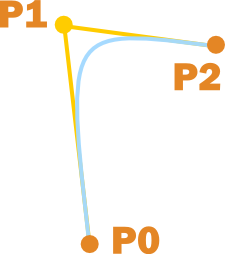
\includegraphics[width=\textwidth,height=6cm,keepaspectratio=true]{bezier_2_devmag}
    \caption{Esquema de una curva Bézier cuadrática de Herman Tulleken, Bézier Curves for your Games: A Tutorial \cite{bezierdevmag_imagen}.}
    \label{fig:basics AFM sketch}
\end{figure}

Hemos usado la función Bézier con tres puntos después de eliminar el zigzag, así que cada tres puntos del A* sin zigzag se usan como puntos de control que servirán para crear la curva. Si los puntos más o menos están alineados, el resultado será una recta suavizada, y si forman una curva, se eliminan los segmentos rectos y se reemplazan con puntos que forman una curva.

\newpage 

La función Bézier cuadrática para tres puntos de control y parámetro t es:

\begin{center}
$[x, y, z] = (1 – t)^2P_0 + 2(1 – t)tP_1 + t^2P_2$
\end{center}

En formato expandido:
\begin{center}
$x = (1 – t)^2x_0 + 2(1 – t)tx_1 + t^2x_2$

$y = (1 – t)^2y_0 + 2(1 – t)ty_1 + t^2y_2$

$z = (1 – t)^2z_0 + 2(1 – t)tz_1 + t^2z_2$
\end{center}

\begin{figure}[htpb]
    \centering
    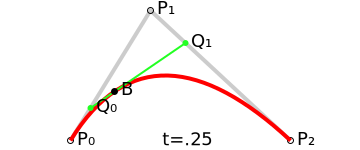
\includegraphics[width=\textwidth,height=6cm,keepaspectratio=true]{Bezier_2_wikipedia}
    \caption{Esquema de una curva Bézier cuadrática de Bézier curve --- Wikipedia \cite{wiki:bezierimagen}.}
    \label{fig:basics AFM sketch}
\end{figure}

\section{Theta*}
Theta A* es un algoritmo desarrollado por A. Nash, K. Daniel, S. Koenig y A. Felner \cite{thetaestrella} que modifica el A* original para obtener rutas más realistas.


\subsection{Pseudocódigo Theta*}


\section{Referencias}

Las referencias se incluyen en el texto usando cite \cite{wiki:latex}. Para citar webs, artículos o libros \cite{koza92}.


\section{Imágenes}

Se pueden incluir imágenes con los comandos standard de \LaTeX, pero esta plantilla dispone de comandos propios como por ejemplo el siguiente:

\imagen{escudoInfor}{Autómata para una expresión vacía}



\section{Listas de items}

Existen tres posibilidades:

\begin{itemize}
	\item primer item.
	\item segundo item.
\end{itemize}

\begin{enumerate}
	\item primer item.
	\item segundo item.
\end{enumerate}

\begin{description}
	\item[Primer item] más información sobre el primer item.
	\item[Segundo item] más información sobre el segundo item.
\end{description}
	
\begin{itemize}
\item 
\end{itemize}

\section{Tablas}

Igualmente se pueden usar los comandos específicos de \LaTeX o bien usar alguno de los comandos de la plantilla.

\tablaSmall{Herramientas y tecnologías utilizadas en cada parte del proyecto}{l c c c c}{herramientasportipodeuso}
{ \multicolumn{1}{l}{Herramientas} & App AngularJS & API REST & BD & Memoria \\}{ 
HTML5 & X & & &\\
CSS3 & X & & &\\
BOOTSTRAP & X & & &\\
JavaScript & X & & &\\
AngularJS & X & & &\\
Bower & X & & &\\
PHP & & X & &\\
Karma + Jasmine & X & & &\\
Slim framework & & X & &\\
Idiorm & & X & &\\
Composer & & X & &\\
JSON & X & X & &\\
PhpStorm & X & X & &\\
MySQL & & & X &\\
PhpMyAdmin & & & X &\\
Git + BitBucket & X & X & X & X\\
Mik\TeX{} & & & & X\\
\TeX{}Maker & & & & X\\
Astah & & & & X\\
Balsamiq Mockups & X & & &\\
VersionOne & X & X & X & X\\
} 
